\phantom\phantomsection
\chapter{Facial expression recognition}

\noindent
\textbf{\color{red} Introductory paragraph of the chapter}

\section{General structure}

\noindent Facial expression recognition is a system enabling an automatic recognition of emotions displayed by a human face. Facial expression recognition can be image or video-based; it can also be computed real-time. Most of the time, researchers try to recognize emotions out of images of human faces. This can also be achieved real-time on video streams : While the person displays his/her emotions, the facial expression recognition system analyses the video, and detect in real-time the displayed emotion.
\newline

\noindent In both cases, facial expression recognition process is structured as follows:


\noindent 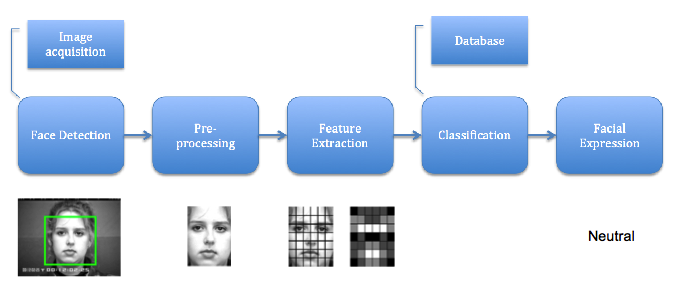
\includegraphics[scale=0.6]{figures/facial_expression_recognition_process}

\subsection{Image Acquisition}

\vspace{\baselineskip}
\noindent First step of the process is "Image Acquisition". Images used for facial expression recognition can be static images or image sequences. Image sequences give more informations about the facial expression, as the steps in muscles movement. About static images, facial expression recognition systems usually need 2D greyscale images as inputs. We can however expect future systems to use colour images; first because of the increasing affordability of technologies and devices capable of capturing images or image sequences; then because colours can give more information on emotions, i.e blushing \cite{CHI03}.
\newline

\subsection{Face Detection}

\vspace{\baselineskip}
\noindent Second step is "Face Detection". Indeed, in a static image and even more in an images sequence, this is an obvious need. Once the face has been detected, all other non-relevant information can be deleted, since only the face is needed. It could hence be included in the next step, which is "Pre-processing", but because of its importance it represents a step in itself. In a real-time facial expression recognition system working with image sequences, the face has to be detected, but also tracked. One of the most used and famous detection and tracking algorithm is the Viola-Jones Algorithm, which we will explain in detail later in this report. This algorithm can be trained to detect all kind of objects, but is mostly used for face detection. 
\newline

\subsection{Pre-processing}

\vspace{\baselineskip}
\noindent Third step is "Pre-processing", which is about applying image processing algorithms to the image, in order to prepare it for the next step. Pre-processing is usually about noise removal, normalization against the variation of pixel position or brightness, segmentation, location, or tracking of parts of the face. Emotion recognition is also sensitive to transformation, scaling and rotation of the head in the image or image sequence. In order to solve this problem, the image can be geometrically standardized. References used for this standardization are usually the eyes \cite{CHI03}.
\newline

\subsection{Features Extraction}

\vspace{\baselineskip}
\noindent Once the image has gone through the "Pre-processing" step, the next one is "Features Extraction". In this step, data is converted into a higher representation of shape, motion, colour, texture, and spatial configuration of the face or its components. One of the main goals of this step is to reduce the dimensionality of the input data. The reduction procedure should retain essential information possessing high discrimination power and high stability \cite{CHI03}. There are a lot of features extraction methods. The most famous are : Principal Component Analysis (PCA), Linear Discriminant Analysis (LDA), Problem Based Learning (PBL), Hidden Markov Models (HMM), Eigenfaces, Gabor Wavelets. The extracted data is then used in the "Classification" step.
\newline

\subsection{Classification}

\noindent
\textbf{\color{red} INSERT PARAGRAPH ON CLASSIFICATION}
- explanation

- existing algorithms : PCA et LDA, mais aussi neural networks, svm

\phantomsection
\section{Existing systems}

\vspace{\baselineskip}
\noindent Before developing a facial expression recognition project, it is important to know what already exist; the state of the art of facial expression recognition system. In this chapter, an overview will be given of the existing systems before to decide on a system for the project.
\textbf{\color{red} Introductory paragraph on which methods are we going to focus on, appearance-based \& geometry-based}
\newline

\subsection{Principal Component Analysis (PCA)}

\vspace{\baselineskip}
\noindent This is a statistical method; one of the most used in linear algebra. PCA is mainly used to reduce high dimensionality of data and to obtain the most important information from this data. Because Facial Expression Recognition needs to reduce the dimensionality of data during features extraction, PCA is commonly used. It helps transforming high dimensionality of data to a new coordinate system of lower dimensions while still preserving the most important information. PCA computes a covariance matrix and a set of values called the eigenvalues and eigenvectors from the original data \cite{GAN08}.
\newline

\subsection{Linear Discriminant Analysis (LDA)}

\vspace{\baselineskip}
\noindent Linear Discriminant Analysis is also a statistical method, used to classify a set of objects into groups. It is done by observing a set of features that describe the objects. LDA as PCA are used to establish a linear relationship between the dimensions of the data. The main difference is that LDA uses the linear relationship to model the differences into classes of objects and PCA does not take any differences into account in the linear relationship. The idea is to perform a linear transformation on the data to obtain a lower dimensional set of features \cite{GAN08}.
\newline

\subsection{Local Binary Patterns (LBP)}

\vspace{\baselineskip}
\noindent This is an appearance-based method. It can be used to describe texture and shape. LBP extracts some informations from the neighbourhood of a central pixel. It compares the intensity values of the neighbourhood pixels with the intensity value of the central pixel  \cite{GAN08}. This method is the one that will be used for this Facial Expression Recognition system.
\newline

\subsection{Hidden Markov Models (HMM)}

\vspace{\baselineskip}
\noindent These models are a set of statistical models used to characterize the statistical properties of a signal (L. Rabiner and B. Huanf, Fundamentals of Speech Recognition. Englewood Cliffs, NJ: Prentice-Hall, 1993.).It is developed to recognize expressions based on the maximum likelihood decision criterion (Automatic Recognition of Facial Expressions Using Hidden Markov Models and Estimation of Expression Intensity Jenn-Jier James Lien April 14, 1998).
\newline

\subsection{Eigenfaces}

\vspace{\baselineskip}
\noindent Eigenfaces
\newline

\subsection{Gabor Wavelets}

\vspace{\baselineskip}
\noindent Gabor Wavelets
\newline

\phantomsection
\section{Issues}

\vspace{\baselineskip}
\noindent bla bla bla
\newline

\phantomsection
\section{Requirements}

\vspace{\baselineskip}
\noindent bla bla bla
\newline


